\chapter{Speichersysteme}

Speichersysteme sind eine entscheidende Komponente der IT Infrastruktur eines Unternehmens. In der heutigen Zeit kann von Speichersystemen kaum abgesehen werden, da Big Data mehr an Wichtigkeit gewinnt. Big Data ist ein Begriff, der sich auf große Mengen an strukturierten, semi-strukturierten und unstrukturierten Daten bezieht, die mit hoher Geschwindigkeit und in unterschiedlichen Formaten generiert, gespeichert und analysiert werden. Diese umfasst Daten, die aus verschiedenen Quellen stammen, wie beispielsweise soziale Medien, Sensoren, Maschinenprotokolle, Transaktionsdaten und Textdokumente. Laut \citeauthor{oracle-bigdata} fallen die bekannten drei V-Begriffe Variety, Volume und Velocity darunter, die im Artikel \glqq Was versteht man unter Big Data?\grqq\ erwähnt werden. Sie bieten eine Möglichkeit, große Mengen an Daten zu speichern und zu verwalten, um den Zugriff und die Nutzung zu erleichtern. Es gibt eine Vielzahl an Speichersystemen, die für verschiedene Zwecke konzipiert sind. Durch die große Auswahl in der IT und die stetig anwachsende Innovation stellt sich die Frage, welche Speichersysteme sich für bestimmte Zwecke eignen. Die Wahl des richtigen Speichersystems hängt von den Anforderungen der Applikation ab, beispielsweise der Art der zu speichernden Daten, dem benötigten Zugriff und der Skalierbarkeit. Eine gründliche Analyse der Anforderungen und Kosten ist entscheidend, um die beste Lösung zu finden, die den Bedürfnissen des Unternehmens entspricht.\\

Im folgenden Kapitel werden die unterschiedlichen Typen von Speichersystemen vorgestellt, wobei der Fokus auf den drei Speicherarten File-, Object- und Block Storage liegt. Im Anschluss daran erfolgt ein Vergleich von zwei Cloud Providern in Bezug auf sichere Speicherung, Hochverfügbarkeit, Performance, Kosten, Integration in Software-Produkte sowie der Dateibereitstellung. Auf Basis dieser Kriterien wird eine Entscheidung darüber getroffen, welcher Provider den Bedürfnissen von leoticket am besten entspricht. Hierbei fließen die Kosten- und Performance-Analysen mit in die Entscheidung ein.

\newpage

\section{Arten von Speichersystemen}
 
Die heutige IT-Landschaft bietet eine Vielzahl von Speichersystemen, die je nach Bedarf und Anforderungen ausgewählt werden können. Neben den traditionellen Speichermedien wie File Storage gibt es andere Arten, die in der Cloud oder als lokale Lösungen bereitgestellt werden können. Dazu gehören unter anderem Object Storage und Block Storage. Jede dieser Speicherarten hat ihre spezifischen Vor- und Nachteile und ist für bestimmte Anwendungsfälle besser geeignet. 
 
\subsection{File Storage}

File Storage, auch dateiebenen- oder dateibasierter Storage genannt \footcite{redHat-storage}, ist eine Speicherlösung bei der Dateien auf einem Dateisystem gespeichert werden. 

\begin{quote}
	Dieses System wird auch als hierarchischer Storage bezeichnet und gilt als das älteste und am weitesten verbreitete Datenspeichersystem für Direct und Network-Attached Storage. Dateisysteme organisieren Daten in hierarchischen Ordnern und Unterverzeichnissen, beispielsweise auf einem Computer. Dateien werden in der Regel auf einem Server oder einer Festplatte gespeichert und können von mehreren Benutzern gleichzeitig gelesen und geschrieben werden. Hierbei werden die Informationen in einzelnen Verzeichnissen abgelegt und können über den entsprechenden Pfad aufgerufen werden. Um dies zu ermöglichen, werden Metadaten genutzt, die dem System den Standort der Dateien mitteilen, vgl. \citeauthor{redHat-storage}.
\end{quote}

In der folgenden Abbildung wird die hierarchische Struktur des Dateispeichers visualisiert.

\begin{figure}[h]
\centering
	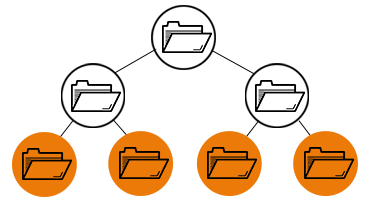
\includegraphics[width=8cm,keepaspectratio]{Pictures/FileStorageHierarchy.png}
	\caption{File Storage: Aufbau des Hierarchiesystems, \citeurl{redHat-storage}}
\end{figure}

File Storage wird häufig in Unternehmen und Organisationen eingesetzt, um gemeinsame Dateiserver bereitzustellen oder Daten in Cloud-Speicherdiensten wie Dropbox oder Google Drive zu speichern.
Auch wenn es von Betriebssystemen und Anwendungen gut unterstützt wird, kann die Performance und Skalierbarkeit von File Storage bei sehr großen Dateisystemen beeinträchtigt werden, was insbesondere bei stark frequentierten Anwendungen oder bei der Verarbeitung großer Datenmengen zum Problem werden kann. 

\newpage

\begin{quote}
	Mit zunehmendem Datenvolumen erfordert das Skalieren von Dateispeichern das Hinzufügen neuer Hardwaregeräte oder den Austausch vorhandener Geräte durch solche mit höherer Kapazität. Dies kann im Laufe der Zeit teuer werden. \glqq As data volumes expand, scaling file storage requires [...]\grqq, (\cite{nx-fileScala}, Übersetzung des Autors)
\end{quote}

Laut Wahlmann (\citeyear{nx-fileScala}, Übersetzung des Autors) wird die Datenspeicherung bei zu vielen Daten nicht nur teuer, sondern auch unhandlich und zeitaufwändig. Der schnelle und einfache Zugriff auf jede Datei wird schwierig, wenn viele Dateien in sehr vielen Verzeichnissen verteilt auf viele Speichermedien gespeichert werden. 

\newpage

\subsection{Block Storage}

Block Storage in der lokalen Umgebung bezieht sich auf die Speicherung von Daten in Form von Speicherblöcken auf physischen Geräten. Im Gegensatz dazu erfordert File Storage ein Dateisystem, das die Organisation, Verwaltung und den Zugriff auf die gespeicherten Daten ermöglicht. Speichermedien ohne ein Dateisystem, wie eine leere Festplatte oder ein nicht formatiertes Laufwerk, können als Block Storage betrachtet werden, da sie die Daten in Blöcken speichern können, ohne eine spezifische Dateiorganisation zu haben.\\

Block Storage in der Cloud speichert Dateien auf Cloud-basierten Speicherumgebungen. Die Cloud-basierte Block Storage stellt dabei einzelne Speicherblöcke als Service bereit. Dies geschieht in Form von virtuellen Festplatten oder Blockvolumes, die über die Cloud-Infrastruktur angeboten werden. Bei der Verwendung von Block Storage in der Cloud können Benutzer Speicherblöcke in beliebiger Größe erstellen und diese an virtuelle Maschinen oder andere Ressourcen in der Cloud anhängen. Der Zugriff auf die Speicherblöcke erfolgt über ein Blockprotokoll wie iSCSI oder Fibre Channel.\\

\begin{quote}
	Wenn auf Block Storage gespeicherte Daten abgerufen werden, verwendet das Server-Betriebssystem die eindeutige Adresse, um die Blöcke wieder zusammenzufügen und so die Datei zu erstellen. Der Vorteil besteht darin, dass das System nicht durch Verzeichnisse und Dateihierarchien navigieren muss, um auf die Datenblöcke zuzugreifen. Dadurch werden Effizienzen erzielt, da der Abruf von Daten schneller erfolgen kann, vgl. \cite{ibm-storage}.
\end{quote}

Typische Anwendungsbereiche des Block Storage sind Datenbanken, Virtualisierungsumgebungen und Anwendungen für Big Data-Analysen. Speicherung von Daten wie Datenbanken, Virtuelle Maschinen und Betriebssysteme eignen sich besonders bei der Verwendung von Block Storage. Sie ermöglichen eine hohe Flexibilität, da Benutzer die Größe und Konfiguration der Speicherblöcke anpassen können, um den individuellen Anforderungen gerecht zu werden. Darüber hinaus bieten sie eine hohe Skalierbarkeit, da zusätzliche Speicherblöcke bei Bedarf hinzugefügt werden können, um den wachsenden Speicherbedarf zu bewältigen. Diese Art von Daten erfordert schnellen und direkten Zugriff auf bestimmte Bereiche des Speichers und muss häufig in Echtzeit ausgeführt werden. Block Storage eignet sich daher am besten für Anwendungen mit hohen Anforderungen an die Leistung und niedriger Latenzzeit.

\newpage

\subsection{Object Storage}

Object Storage hat sich als Speichertechnologie in den letzten Jahren immer stärker etabliert und wird von vielen Unternehmen als Alternative zu traditionellen Speicherlösungen wie Block- oder File Storage angesehen. Die ersten Object Storage Systeme wurden bereits in den 1990er Jahren entwickelt, aber erst mit dem Aufkommen von Big Data, IoT und der Cloud-Nutzung 
 hat es einen breiteren Einsatz gefunden. Heute bieten viele Cloud Provider wie Amazon Web Services (AWS) und Google Cloud Platform (GCP) Object Storage als einen ihrer Haupt-Cloud-Services an.
 
\begin{quote}
	Object Storage ist für den Umgang mit großen Datenvolumen und unstrukturierten Daten entwickelt. Sie speichert Daten als eigenständige Objekte, die aus Daten und Metadaten bestehen und einen eindeutigen Identifier (UID) haben, (\glqq Object storage (aka object-based storage) is a type of data storage used to [...]\grqq, \cite{dataCore-OS}, Übersetzung des Autors).
\end{quote}

Im Gegensatz zu hierarchischen Systemen wie beim File Storage ist das Speichersystem flach strukturiert. Durch die einfache API Anbindung kann es mit vorhandenen Anwendungen integriert werden. Nutzer können detaillierte Informationen wie beispielsweise Erstellerangaben, Schlüsselwörter sowie Sicherheit-und Datenschutzrichtlinien hinterlegen. Diese Daten bezeichnet man als Metadaten. Laut \citeauthor{nx-fileScala}, 2022 ist Skalierbarkeit der Hauptvorteil, da bei der Speicherung von Petabyte und Exabyte alle Objekte in einem Namespace abgelegt werden. Selbst wenn dieser Namespace auf Hunderten von Hardwaregeräten und Standorten verteilt ist, können alle Objekte schnell abgerufen werden. Ein weiterer Vorteil von Objekt Storage beinhaltet die Fehlercodierung bzw. Fehlerkorrekturverfahren, im Englischen bekannt als \glqq Erasure Coding\grqq.\\

Auch Object Storage hat Nachteile. Laut \citeauthor{redHat-storage} muss das Objekt nach der Speicherung bei Veränderung komplett neu überschrieben werden. Sie sind für traditionelle Datenbanken nicht geeignet, da das Schreiben von Objekten Zeit beansprucht und die Implementierung einer Applikation für die Nutzung der Object Storage API ist aufwendiger als die Nutzung von File Storage, vgl. \citeauthor{redHat-storage}.\\

Insgesamt bietet Object Storage eine skalierbare und flexible Methode zur Speicherung von unstrukturierten Daten. Organisationen sollten jedoch die Vor- und Nachteile von Object Storage im Kontext ihrer spezifischen Anwendungsfälle abwägen, um eine fundierte Entscheidung über die beste Speichermethode zu treffen.\\


\textbf{Fazit}\\

Aufgrund der Anforderungen von leoticket, Daten wie Rechnungen und Tickets zu speichern und abzurufen, erweist sich Object Storage als die geeignete Speicheroption. Da keine spezifischen Anforderungen hinsichtlich der Latenzzeit bestehen und auch keine Dateien im Petabyte- oder Exabyte-Bereich gespeichert werden müssen, scheidet die Block Storage-Variante aus. Viele Cloud-Anbieter stellen Methoden für Object Storage bereit, die Sicherheitsfunktionen, hohe Verfügbarkeit, gute Performance und eine Möglichkeit der Integration in Software-Produkten umfassen. Darüber hinaus ermöglichen Object Storage-Systeme die Bereitstellung von Dateien als Links. Die Skalierbarkeit ist ein weiterer entscheidender Faktor, der für die Wahl von Object Storage spricht.

\newpage

\section{Aktuelle Speichertechnologien im Markt}

Die beiden bekanntesten Cloud-Anbieter Amazon Web Services (AWS) und Google Cloud Platform (GCP) bieten eine Vielzahl von Speicherlösungen an, die auf die Bedürfnisse von Unternehmen zugeschnitten sind.\\ 

In diesem Kapitel werden die aktuellen Speichertechnologien auf dem Markt untersucht, wobei der Fokus auf den Angeboten von AWS und GCP liegt. Um eine Vergleichsgrundlage zwischen AWS und GCP zu schaffen, werden die verschiedenen Aspekte wie sichere Speicherung, Hochverfügbarkeit, Leistung, Kosten, API Anbindung und die Bereitstellung der Dateien betrachtet. Dieses Vorgehen dient der Ermittlung der angebotenen Object Storage Speichersysteme der Cloud Provider, die am besten die genannten Anforderungen erfüllen.\\

AWS bietet eine Reihe von Speicheroptionen an, darunter Amazon S3 (Simple Storage Service). Amazon S3 ist ein Object Storage-Service, der für die Speicherung und den schnellen Abruf von unstrukturierten Daten wie Videos, Fotos und Dokumenten ausgelegt ist. GCP stellt mit Google Cloud Storage (GC Storage) unter anderem eine ähnliche Speicherlösung bereit. Diese ist ein Object-Storage-Service, der für die Speicherung selbiger Daten optimiert ist.\\

\subsection{Eigenschaften}

Im folgenden Abschnitt werden Amazon S3 und GC Storage in Bezug auf verschiedene Kriterien untersucht. Die Auswahl der Kriterien erfolgt in Anlehnung an die spezifischen Anforderungen von leoticket. Dabei werden zunächst die Eigenschaften von Amazon S3 erläutert, gefolgt von einer Betrachtung von GC Storage. Ziel ist es, Funktionen und Angebote beider Cloud Provider zu untersuchen, um eine Entscheidungshilfe für leoticket zu bieten. 

\newpage

\subsubsection{Sichere Speicherung}

Viele Anbieter von Object Storage-Lösungen bieten integrierte Verschlüsselungsmöglichkeiten an, um sicherzustellen, dass Daten sowohl während der Übertragung als auch in Persistenz geschützt sind. Dabei können unterschiedliche Verschlüsselungsmethoden zum Einsatz kommen. In Bezug auf die sichere Speicherung bieten sowohl AWS als auch GCP Optionen für die Verschlüsselung von Daten. Die Sicherheit der gespeicherten Daten ist von entscheidender Bedeutung, um ihre Vertraulichkeit zu gewährleisten und den Zugriff auf sie einzuschränken.\\

\textbf{Amazon S3}\\

IAM (Identity and Access Management) ist ein essentieller Bestandteil von AWS und ermöglicht Benutzer, Gruppen und Rollen zu erstellen, um den Zugriff auf S3 zu verwalten. Benutzern können individuelle Berechtigungen zugewiesen werden, während Gruppen und Rollen mehrere Benutzer mit denselben Berechtigungen zusammenfassen können. Auf S3-Buckets und Objekte kann eine granulare Zugriffssteuerung angewendet werden. Benutzer, Gruppen oder Rollen können so konfiguriert werden, den Zugriff auf bestimmte Buckets und Objekte zu erlauben. "Beim Erteilen von Berechtigungen in Amazon S3 entscheiden Sie, wer die Berechtigungen erhält, für welche Amazon-S3-Ressourcen die Berechtigungen gelten und welche Aktionen zu diesen Ressourcen gestattet werden sollen."\cite{aws-iam-s3}\\

Eine weitere Sicherheitsfunktion von Amazon S3 ist die Datenverschlüsselung. S3 bietet eine Vielzahl von Verschlüsselungsoptionen für die serverseitige und clientseitige Verschlüsselung. Da die clientseitige Verschlüsselung für leoticket keine Anwendung findet, wird diese Methode nicht weiter in Betracht gezogen. Die clientseitige Verschlüsselung erfordert die Generierung und Kommunikation eines separaten Schlüssels für jeden Kunden, um auf die Dateien zugreifen zu können. Aus Gründen des Aufwands ist diese Vorgehensweise nicht praktikabel. Daher wird der Schwerpunkt auf die serverseitige Verschlüsselung gelegt. Es existieren drei Verschlüsselungsmethoden: die serverseitige Verschlüsselung mit Amazon S3-verwalteten Schlüsseln (SSE-S3), mit dem AWS Key-Management-Service-verwalteten Schlüsseln (SSE-KMS) und die vom Kunden verwalteten Schlüsseln (SSE-C). Durch diese Optionen haben Benutzer die Möglichkeit, die Verschlüsselung gemäß ihren individuellen Anforderungen anzupassen und somit die Datensicherheit zu gewährleisten.\\

Laut \citeauthor{aws-iam-s3} nutzen Buckets standardmäßig die SSE-S3 Methode. Für die Verschlüsselung wird 256-bit Advanced Encryption Standard (AES-256) verwendet. Seit dem 5. Januar 2023 sind alle neu erstellen Buckets auf SSE-S3 ausgelegt. Alle neuen Objekte sind beim Hochladen ohne weitere Zusatzkosten und Einbußen der Leistung automatisch verschlüsselt.

\begin{quote}
	Die Serverseitige Verschlüsselung schützt die Daten bei der Übertragung von und nach S3, ebenso wenn sie auf den Datenträgern in S3-Rechenzentren gespeichert sind. Amazon S3 verschlüsselt jedes Objekt mit einem eindeutigen Schlüssel. Als zusätzliche Sicherheitsmaßnahme werden diese eindeutigen Schlüssel mit einem weiteren Schlüssel verschlüsselt, welches in regelmäßigen Abständen rotiert wird, vgl. \cite{aws-iam-s3}
\end{quote}

\newpage

Amazon S3 bietet auch die SSE-KMS (Server-Side Encryption with AWS Key Management Service) als Option an. AWS-KMS ist ein Dienst, der ein Schlüsselverwaltungssystem zur Verfügung stellt. Es verschlüsselt die Objektdaten und speichert die S3-Prüfsumme, die sich in den Objektmetadaten befindet, in verschlüsselter Form. Die SSE-KMS kann über die AWS Management-Konsole oder die AWS KMS API verwaltet werden.\\

Bei der Verwendung von SSE-KMS stehen zwei Methoden zur Verfügung: AWS-Managed-Key oder Customer-Managed-Key. Diese unterstützen die sogenannte \glqq envelope encryption\grqq. Das bedeutet, dass die Schlüssel für die Daten mithilfe eines Master Keys verschlüsselt werden. Dies erleichtert die Verwaltung der Schlüssel.\\

Bei der Verwendung der AWS-Managed-Key-Variante wird automatisch ein Schlüssel generiert, sobald ein Objekt in einen Bucket hochgeladen wird. Dieser generierte Schlüssel wird anschließend für die Ver- und Entschlüsselung der Daten verwendet. Wenn jedoch ein eigener Schlüssel über KMS verwendet werden soll, muss zunächst ein symmetrischer Schlüssel vor der KMS-Konfiguration erstellt werden. Bei der Erstellung des Buckets kann danach der selbst erstellte Schlüssel angegeben werden. Die Verwendung von Customer-Managed-Keys bietet bestimmte Vorteile, die den Anforderungen von leoticket entsprechen. Durch die Verwendung von selbst erstellten Schlüsseln wird mehr Flexibilität und Kontrolle gewährleistet. Diese Schlüssel können selbst erstellt, rotiert und deaktiviert werden. Zusätzlich können Zugriffskontrollen und Auditierung konfiguriert werden, um den Schutz der Daten zu gewährleisten.\\

Durch die Auswahl der SSE-KMS-Variante besteht die Möglichkeit, die S3 Bucket Key-Funktion zu aktivieren. Diese Funktion kann die Anfragekosten um bis zu 99 Prozent reduzieren, indem der Anfragenverkehr von Amazon S3 zu AWS KMS verringert wird. Durch die Aktivierung des S3 Bucket Keys werden eindeutige Datenschlüssel für die Objekte im Bucket generiert. Diese Bucket Keys werden für einen festgelegten Zeitraum verwendet, wodurch die Anfragen an Amazon S3 zur Durchführung von Verschlüsselungsoperationen auf AWS KMS reduziert werden.\\

Die letzte Option ist SSE-C (Server-Side Encryption with Customer-Provided Keys). Bei SSE-C stellt der Kunde seinen eigenen Schlüssel zur Verfügung. Im Gegensatz zu AWS KMS speichert Amazon S3 diesen Schlüssel nicht. Mit dem bereitgestellten Schlüssel übernimmt Amazon S3 die Datenverschlüsselung während des Schreibvorgangs sowie die Datenentschlüsselung beim Zugriff auf Objekte. Anschließend entfernt Amazon S3 den Schlüssel aus dem Speicher. Da Amazon S3 den Schlüssel nicht speichert, wird der zufällig generierte HMAC (Hash-based Message Authentication Code) des Verschlüsselungsschlüssels gespeichert, um zukünftige Anfragen zu validieren. \glqq Note: Amazon S3 does not store the encryption key that you provide.\grqq, \cite{aws-sse-c}.

\newpage

Object Ownership ist eine weitere Sicherheitsfunktion von Amazon S3. Mit Object Ownership können Benutzer oder Gruppen die Eigentümerschaft von Objekten in S3-Buckets besitzen. Dies bedeutet, dass nur autorisierte Benutzer die Berechtigung haben, Objekte zu löschen oder zu ändern, was die Sicherheit der Daten erhöht. \glqq S3 Object Ownership ist eine Einstellung auf Amazon-S3-Bucket-Ebene, mit der Sie Zugriffskontrolllisten (ACLs) deaktivieren und das Eigentum an jedem Objekt in Ihrem Bucket übernehmen können, [...].\grqq, \cite{aws-iam-s3}.\\

AWS empfiehlt die ACL (Access Control List) auf Bucket-Ebene deaktiviert zu lassen. Alle Objekte eines Buckets gehören so dem Bucket Owner. Laut \citeauthor{aws-iam-s3} verfügt Object Ownership über drei Einstellungen, mit denen man die Eigentümerschaft von Objekten steuern kann.

\begin{table}[!h]
\begin{tabular}{ |p{2cm}|p{2.1cm}|p{2.6cm}|p{2.6cm}|p{2.5cm}| }
\hline
\textbf{Einstellung} & \textbf{Gilt für} & \textbf{Auswirkung auf Object Ownership} & \textbf{Auswirkungen auf ACLs} & \textbf{Hochladen akzeptiert} \\
\hline
Bucket-Eigentümer erzwungen(empfohlen) & Alle neuen und bestehenden Objekte & Bucket-Eigentümer besitzt jedes Objekt. & ACLs sind deaktiviert. Bucket-Eigentümer hat das volle Eigentum und die volle Kontrolle. & Uploads mit ACL mit vollem Zugriff des Bucket-Eigentümers oder Uploads, die keine ACL angeben \\
\hline
Bucket-Eigentümer bevorzugt & Neue Objekte   & Wenn ein Objekt-Upload die bucket-owner-full-control vordefinierte ACL beinhaltet, gehört dem Bucket Eigentümer das Objekt. Objekte, die mit anderen ACLs hochgeladen wurden, gehören dem Schreibkonto & ACLs können aktualisiert werden und können Berechtigungen erteilen. Wenn ein Objekt-Upload die bucket-owner-full-control vordefinierte ACL enthält, hat der Bucket-Eigentümer Vollzugriff und der Objekt-Writer hat keinen Vollzugriff mehr. & Alle Uploads \\
\hline
Object-Writer (Standard) & Neue Objekte & Der Objekt-Writer besitzt das Objekt & ACLs können aktualisiert werden und können Berechtigungen erteilen. Der Objekt-Writer hat vollen Kontrollzugriff & Alle Uploads \\
\hline
\end{tabular}
\caption{Einstellungen für Object Ownership, \citeurl{aws-iam-s3}}
\end{table}


Laut \citeauthor{aws-iam-s3} zeigt die obige Tabelle die Auswirkungen, die jede Einstellung für Object Ownership auf ACLs, Objekte, Objekteigentümer und Objekt-Uploads hat.\\

Logging ist ein weiterer Aspekt der Amazon S3-Sicherheit. S3 bietet Logging-Optionen, darunter Bucket Logging und Object-Level Logging, die es Benutzern ermöglichen, Zugriffe auf S3-Objekte aufzuzeichnen und zu überwachen. Diese Funktionen sind entscheidend, um verdächtige Aktivitäten zu erkennen. AWS bietet eine Vielzahl von Tools zur Überwachung der Amazon S3 Ressourcen. Darunter die Amazon CloudWatch Alarms, AWS CloudTrail Logs, Amazon S3 Access Logs und die AWS Trusted Advisor.\\

\newpage

\textbf{Google Cloud Storage}\\

Mit Cloud IAM können ähnlich wie in AWS IAM auch rollenbasierte Zugriffsberechtigungen auf bestimmte Ressourcen beispielsweise für Bucket-, und Objektebene umgesetzt werden. Sowohl Rollen als Berechtigungen können in ähnlicher Funktionsweise wie bei AWS erstellt und zugewiesen werden. GC IAM verwendet das Konzept von Rollen, um Berechtigungen zu definieren. Es bietet vordefinierte Rollen wie Besitzer, Bearbeiter und Viewer, die verschiedene Berechtigungen für bestimmte Ressourcen gewähren. AWS IAM verwendet ebenfalls Rollen, um Berechtigungen zu definieren. Es bietet vordefinierte Rollen wie Administratorzugriff und Lesezugriff. Es ist zu beachten, dass beide Dienste unterschiedliche Terminologien und Konzepte verwenden können, obwohl sie ähnliche Funktionen bieten.\\

Auch GC bietet eine Vielzahl an Sicherheitsfunktionen, um sicherzustellen, dass Daten in der Cloud sicher gespeichert und geschützt sind. Unter anderem die Datenverschlüsselung. GC bietet wie Amazon S3 die serverseitige Verschlüsselung an. Hier werden zwischen Google-managed Keys, Customer-managed encryption keys und die Customer-supplied encryption keys unterschieden. Google-managed encryption ist die Standard Verschlüsselungsoption von GC ähnlich wie die AWS SSE-S3. AWS und GC bieten ähnliche Funktionalitäten der Datenverschlüsselung an. Dies wäre die serverseitige Datenverschlüsselung, bevor die Daten auf die Festplatte geschrieben werden. 

\begin{quote}
	Die Standard Variante verwaltet für den Nutzer die Encryption Keys in ihrem eigenen Key Management System. Auch GC verwendet für die Verschlüsselung die AES-256 wie AWS. Als Nutzer muss man bei dieser Variante keine Einstellungen berücksichtigen. Daten werden automatisch beim Abruf entschlüsselt, vgl. \cite{gcp-encrypt}.
\end{quote}

Wenn ein höheres Maß an Kontrolle über die Schlüssel gewünscht wird, steht die Option der Customer-Managed Encryption zur Verfügung, die mit der AWS SSE-KMS customer-managed-Funktion gleichwertig ist. Die Schlüssel werden durch den Cloud KMS (Cloud Key Management Service) erstellt und verwaltet. Der Benutzer speichert diese Schlüssel extern oder in einem HSM-Cluster (Hardware Security Module). Customer-Keys können entweder für einzelne Objekte verwendet werden oder es kann ein Standard-Key für einen Bucket erstellt werden. Ähnlich wie bei den Bucket Keys in AWS können die erstellten Schlüssel zur Verschlüsselung der Objektdaten, zur CRC32C-Prüfsumme des Objekts und für den MD5-Hash verwendet werden. Um zusätzlichen Schutz zu gewährleisten, stehen Service Agents zur Verfügung, auch bekannt als Service Accounts. Diesen Agenten können bestimmte Berechtigungen zugewiesen werden, um Zugriff auf den gewünschten Encryption Key zu erhalten und Objekte zu verschlüsseln.\\


Schließlich besteht auch die Möglichkeit der Verwendung von Customer-supplied Encryption Keys, vergleichbar zu AWS SSE-C-Variante. Als zusätzliche Sicherheitsebene zu Google-managed encryption keys können Nutzer ihren eigenen AES-256 Encryption Key bereitstellen, welcher in Base64 encoded ist. Bei dieser Variante wird der Schlüssel nicht von GC gespeichert oder verwaltet. Genau wie bei AWS SSE-C müssen die Nutzer diese Schlüssel selber verwalten und speichern. Um zukünftige Requests zu validieren speichert GC einen kryptografischen Hash vom Schlüssel. Jedoch kann der Encryption Key nicht aus dem Hash regeneriert werden.\\

Darüber hinaus bietet GC auch Zugriffskontrolleinstellungen, mit denen Benutzer genau steuern können, wer auf Dateien in Buckets zugreifen kann. Der Zugriff kann sowohl auf Bucket- als auch auf Objektebene gesteuert werden, wobei Benutzern und Gruppen bestimmte Rollen zugewiesen werden können. Dabei wird zwischen \glqq Uniform Access Control\grqq\ (UAC) und \glqq Fine-grained Access Control\grqq\ (FGAC) unterschieden. UAC ermöglicht es, ähnlich wie bei der ACL auf Bucket-Ebene in AWS, den Zugriff auf einen gesamten Bucket in GC Storage auf der Ebene von Rollen zuzuweisen. Dabei können verschiedene vordefinierte Rollen wie Leser, Schreiber oder Besitzer verwendet werden, um festzulegen, welche Aktionen ein Benutzer auf dem Bucket ausführen darf. UAC stellt im Gegensatz zu FGAC eine einfachere Methode zur Zugriffskontrolle dar, da die Zugriffsrechte auf Bucket-Ebene vergeben werden. Das bedeutet, dass alle Objekte des Buckets automatisch dieselben Zugriffsrechte erhalten.\\

FGAC hingegen ermöglicht es, die Zugriffskontrolle auf die Ebene von Objekten oder sogar auf Teile von Objekten herunterzubrechen. Das bedeutet, dass jeder Benutzer oder jede Gruppe individuelle Zugriffsrechte auf bestimmte Objekte oder Teile von Objekten haben kann. Mit FGAC können feingranulare Zugriffssteuerungen implementiert werden. Es ist eine mächtige Methode, aber auch komplexer und zeitaufwändiger zu implementieren als UAC. Beide Cloud Provider empfehlen die ACL auf Objekt-Ebene deaktiviert zu lassen und nur bei speziellen Fällen anzuwenden. Standardmäßig ist die ACL auf Bucket-Ebene eingestellt.\\

Für das Object Logging in GC Storage stehen verschiedene Methoden zur Verfügung. GC bietet die Möglichkeit, spezielle Logging-Buckets zu erstellen, in denen alle Zugriffsprotokolle für Objekte gespeichert werden. Auch können Storage-Bucket-Audit-Logs aktiviert werden, um detaillierte Informationen über die Aktivitäten in Buckets zu erhalten.

\newpage

\subsubsection{Hochverfügbarkeit}

\textbf{Amazon S3}\\

Amazon S3 ist ein skalierbarer und hochverfügbarer Object Storage, der eine Verfügbarkeit von 99.99\% garantiert. \glqq Designed to provide 99.999999999\% durability and 99.99\% availability of objects over a given year.\grqq, \cite{aws-availability}\\

Dies wird durch die Verwendung von Multi-Availability Zone Architekturen erreicht, die eine automatische Replikation von Daten in verschiedenen physischen Standorten ermöglichen. Die Multi-Availability Zone Architektur von Amazon S3 basiert auf der Aufteilung von Daten in mehrere geografisch getrennte Verfügbarkeitszonen (AZs). Jede AZ besteht aus mehreren physischen Rechenzentren, die sich in einem geografisch getrennten Gebiet befinden. Jede AZ ist vollständig unabhängig und bietet eine hohe Redundanz und Verfügbarkeit. Wenn ein Benutzer ein Objekt in Amazon S3 hochlädt, wird es automatisch in mehrere AZs repliziert, um sicherzustellen, dass das Objekt auch bei Ausfällen in einer AZ weiterhin verfügbar ist. Im Falle eines Ausfalls einer AZ wird Amazon S3 automatisch die Anfragen auf eine andere AZ umleiten, um eine ununterbrochene Verfügbarkeit des Objekts sicherzustellen. Durch die Cross-Region Replikation (CRR) werden Daten automatisch in andere AWS-Regionen repliziert. Dadurch kann eine hohe Verfügbarkeit der Daten im Falle eines Ausfalls einer gesamten AWS-Region gewährleistet werden. Die Same-Region-Replikation (SRR) funktioniert, ähnlich wie die CRR, nur das hier die Daten in einer einzelnen Region auf die verfügbaren AZs repliziert werden.\\

Zusätzlich zu Multi-Availability Zone Architekturen verwendet Amazon S3 auch Fehlerkorrektur- und Erkennungsmechanismen wie CRC-Prüfungen, um die Integrität von Daten sicherzustellen, damit die gespeicherten Daten stets korrekt sind.\\

Durch Aktivierung der Versionierung wird jeder Objektversion, die in einem S3-Bucket gespeichert ist, eine eindeutige Versions-ID zugewiesen. Wenn eine Objektversion versehentlich gelöscht oder überschrieben wird, kann die vorherige Version wiederhergestellt werden.\\

Um eine hohe Verfügbarkeit bereitzustellen, stellt S3 außerdem noch die S3-Transfer Acceleration zur Verfügung. Durch die Verwendung von Amazon S3-Transfer Acceleration können Benutzer die Übertragung großer Datenmengen beschleunigen, indem ein optimierter Netzwerkpfad genutzt wird. Dadurch kann die Verfügbarkeit der Daten verbessert werden, indem Verbindungsprobleme minimiert werden. Um die Leistung von S3 zu überwachen und auf mögliche Probleme reagieren zu können wird CloudWatch bereitgestellt. Auf diese Weise kann die Ausfallzeit minimiert und analysiert werden, zu welchen Zeitpunkten die Verfügbarkeit am geringsten ist.\\

Insgesamt bietet Amazon S3 eine hochverfügbare und zuverlässige Speicherlösung, die durch Multi-Availability Zone Architekturen und Fehlerkorrekturmechanismen eine Verfügbarkeit von 99,99\% gewährleistet.

\newpage

\textbf{Google Cloud Storage}\\

Laut \cite{gcp-sla} wird die Verfügbarkeit als Service Level Agreement (SLA) angegeben, welches die garantierte Verfügbarkeit des Dienstes definiert. Gemäß dem aktuellen SLA von GC Storage beträgt die garantierte Verfügbarkeit für Multi-Regionale Speicher 99,95\% und für Regionale Speicher 99,9\%. Diese Zahlen geben an, dass GC Storage darauf ausgelegt ist, eine sehr hohe Verfügbarkeit zu gewährleisten. AWS bietet ähnliche Verfügbarkeiten an. Beide versprechen eine nahezu lückenlose Verfügbarkeit. In der folgenden Tabelle werden diese Werte nochmals gezeigt:

\begin{table}[!h]
\centering
\begin{tabular}{ |p{5cm}|p{5cm}| }
\hline
Cloud Service & Monthly Uptime Percentage \\
\hline
\cline{1-2}
Standard storage class in a multi-region or dual-region location of Cloud Storage & $>$=99.95\% \\
\cline{1-2}
Standard storage class in a regional location of Cloud Storage; Nearline, Coldline, or Archive storage class in a multi-region or dual-region location of Cloud Storage & $>$=99.9\% \\
\cline{1-2}
Nearline, Coldline, or Archive storage class in a regional location of Cloud Storage; Durable Reduced Availability storage class in any location of Cloud Storage & $>$=99.0\% \\
\cline{1-2}
\end{tabular}
\caption{Verfügbarkeit der Speicherklassen gemäß Google Cloud Storage SLA, \citeurl{gcp-sla}}
\end{table}

Es ist jedoch zu beachten, dass die tatsächliche Verfügbarkeit von GC Storage und Amazon S3 von mehreren Faktoren abhängt, einschließlich der spezifischen Konfiguration, dem Datenzugriffsmuster, der Netzwerkverfügbarkeit und anderen betrieblichen Variablen. Es ist daher möglich, dass die tatsächliche Verfügbarkeit in der Praxis leicht von der garantierten Verfügbarkeit abweicht.\\

Auch Google Cloud Storage bietet die Multi-Region Storage wie die CRR von AWS an. Dies ermöglicht die Speicherung von Daten in mehreren Regionen weltweit. Dadurch werden die Daten redundant repliziert und bleiben auch im Falle eines Ausfalls einer Region verfügbar. Dieses Prinzip ähnelt dem von AWS, denn auch dort werden die Daten automatisch repliziert. Außerdem bietet GC genau wie AWS SRR die Single-Region Replikation an.\\

Ein weiterer Punkt ist das Monitoring und Fehlererkennung wie z.B. Stackdriver Monitoring, um die Leistung und Verfügbarkeit von GC Storage zu überwachen und auf potenzielle Probleme zu reagieren. Dies gleicht auch dem CRC von AWS.\\

Zuletzt bietet Object Versioning die Möglichkeit, Objektversionen beizubehalten. Dadurch können vorherige Versionen von Objekten wiederhergestellt werden, falls sie versehentlich gelöscht oder überschrieben werden. Diese Funktionalität entspricht der Objektversionierung von AWS.\\


\subsubsection{Kosten}

In diesem Abschnitt erfolgt eine Untersuchung der Kostenstruktur von Amazon S3 und GC Storage. Dabei werden die generellen Kostenfaktoren betrachtet, für die Cloud-Anbieter Gebühren erheben. Die Angebote der Free Tier Kontingenten werden dabei nicht betrachtet.\\

\textbf{Amazon S3}\\

Amazon S3 erhebt Gebühren für verschiedene Leistungsbereiche, darunter die Speicherung, Anfragen, Datenabrufe, Datenübertragung, Verwaltung, Analyse und Replikation. Die Speicherungsgebühr richtet sich nach der Objektgröße, der Speicherdauer innerhalb eines Monats und der gewählten Speicherklasse. Es stehen verschiedene Speicherklassen zur Verfügung, die für unterschiedliche Anwendungsfälle geeignet sind. Dies sind S3 Standard, S3 Intelligent-Tiering (IA), S3 Standard – Infrequent Access (IA), S3 One Zone – Infrequent Access (IA), S3 Glacier Instant Retrieval, S3 Glacier Flexible Retrieval (ehemals S3 Glacier) und S3 Glacier Deep Archive. In dieser Arbeit wird S3 Glacier nicht behandelt, da die Abrufzeiten der Objekte zu lange Zeit in Anspruch nehmen, was den Anforderungen von leoticket nicht entspricht. Stattdessen werden die Speicherklassen S3 Standard, S3 IA, S3 Standard - IA und S3 One Zone - IA näher untersucht. Zur Veranschaulichung werden die Preise in der folgenden Tabelle dargestellt:

\begin{table}[!h]
\begin{tabular}{ |s|p{2cm}|p{2.5cm}|p{2cm}|p{2cm}| }
\hline
\rowcolor{blue!35}
 & \textbf{Standard} & \textbf{Intelligent Tiering} & \textbf{Standard-IA} & \textbf{One Zone-IA}\\
\hline
\textbf{Speicher/GB im Monat} & 0,023 EUR & 0,023 EUR & 0,013 EUR & 0,010 EUR \\
\textbf{PUT-,COPY-,POST-,LIST-Anforderungen (pro 1000)} & 0,0050 EUR & 0,0050 EUR & 0,0093 EUR & 0,0093 EUR \\
\textbf{GET-,SELECT und alle anderen Anforderungen (pro 1000)}   & 0,00040 EUR & 0,00040 EUR  & 0,00093 EUR & 0,00093 EUR\\
\textbf{Datenwieder-herstellung}  &-- & --  & 0,00093 EUR & 0,00093 EUR\\
\textbf{Monitoring und Automation pro Objekt} & -- & 0,0000023 EUR & -- & --\\
\hline
\textbf{Datenübertragung aus S3 in das Internet} & \multicolumn{3}{c}{0,084 EUR pro GB} &\\
\hline
\end{tabular}
\caption{Übersicht der Kosten der AWS S3 Speicherklassen}
\end{table}

In der vorliegenden Tabelle sind die Standardpreise für verschiedene Speicherklassen von Amazon S3 aufgeführt. Die Preise für PUT-, COPY-, POST- und LIST-Anforderungen basieren auf einer Staffelung von 1000 Anfragen, ähnlich wie bei GET-, SELECT- und anderen Anforderungen.\\

Sowohl die Speicherklasse Standard als auch Intelligent Tiering (IA) haben eine Speicherungsgebühr von 0,023 Euro und Anforderungsgebühren von 0,0050 Euro für POST-Anforderungen und 0,00040 Euro für GET-Anforderungen. Für die Speicherklassen Standard-IA und OneZone-IA liegen die Speicherungsgebühren bei 0,013 Euro bzw. 0,010 Euro. Die Anforderungsgebühren betragen 0,0093 Euro für POST-Anforderungen und 0,00093 Euro für GET-Anforderungen. Zusätzlich erheben beide Speicherklassen eine Datenwiederherstellungsgebühr von 0,00093 Euro. Es fallen auch Datenübertragungsgebühren von Amazon S3 zum Internet in Höhe von 0,084 Euro pro GB für alle Speicherklassen an. Es sei darauf hingewiesen, dass nur die IA-Speicherklasse zusätzliche Gebühren in Höhe von 0,0000023 Euro pro Objekt für das Monitoring und Verwaltung von Objekten erhebt.\\

Auch für die Replikation fallen in Amazon S3 Gebühren an. Bei der Replikation von Daten fallen zusätzlich zu den Speicherungskosten Kosten für die primäre Kopie der Daten, für Replikations-PUT-Anforderungen und Speicherabruf an. Bei CRR wird auch für den regionenüber-greifenden Datentransfer OUT von S3 zu jeder Zielregion gezahlt. Die Preise für Speicher- und PUT-Anfragen für die replizierte Kopie basieren auf den ausgewählten AWS-Zielregionen, während die Preise für Datenübertragungen zwischen den Regionen auf der AWS-Quellregion basieren. Wenn man S3 Replication Time Control nutzt, wird eine Datenübertragungsgebühr für die Replikationszeitsteuerung sowie Gebühren für S3-Replikationsmetriken erhoben, die zum selben Tarif abgerechnet werden wie angepasste Amazon-CloudWatch-Metriken. Die Kosten für die S3 Replication Time Control-Datenübertragung beträgt pro GB 0.015 USD. Unter \href{https://aws.amazon.com/de/s3/pricing/}{AWS Preise} können diese Informationen abgerufen werden.\\

Im Zusammenhang mit der Objektversionierung entstehen Kosten für die Beibehaltung älterer Versionen von Objekten, da zusätzlicher Speicherplatz benötigt wird. Es fallen keine direkten Kosten für das Tagging von benutzerdefinierten Metadaten an, die den Objekten zugeordnet sind. Es ist jedoch möglich, dass Kosten für das Abrufen von Tags über die S3-API (z.B. mit den ListObjects- oder GetObject-Operationen) anfallen, da dies als Datenabruf betrachtet wird und entsprechende Gebühren gemäß den AWS-Preisen für Datenzugriff erhoben werden.\\

Die genauen Preise und Kostendetails für S3 können sich im Laufe der Zeit ändern. Es wird empfohlen, die aktuellsten Informationen auf der offiziellen AWS-Preisseite oder im AWS-Kostenrechner unter \href{https://calculator.aws/}{AWS Calculator} zu überprüfen, um eine grobe Kosteneinschätzung zu erhalten.

\newpage

\textbf{GC Storage}\\

GCS setzt Preise für die Komponenten Datenspeicher, Datenverarbeitung und Netzwerknutzung. Beim Datenspeicher ist, wie bei Amazon S3, die Menge der in Buckets gespeicherten Daten relevant. Preise für Speicher hängen von der Speicherklasse der Daten und dem Standort der Buckets ab. Bei der Verarbeitung werden Gebühren für die von Cloud Storage durchgeführte Verarbeitung, einschließlich Vorgangsgebühren der Klasse A und B, Abrufgebühren und Replikation zwischen Regionen erhoben. Die Vorgangsgebühren der Klasse A beinhalten die PUT-Anforderungen während die Klasse B die GET-Anforderungen beinhalten. Bei der Netzwerknutzung werden Gebühren für die Menge der aus den Buckets gelesenen oder zwischen diesen verschobenen Daten erhoben. GC Storage bietet vier Speicherklassen an, von denen drei untersucht werden. Diese sind die Standard-, Nearline-, und Coldline Storage Klassen. Diese drei Speicherklassen haben unterschiedliche Leistungseigenschaften und Kosten. Die Archive Storage Speicherklasse wird dabei nicht berücksichtigt, da sie hauptsächlich der Archivierung von Daten ausgelegt ist und dem leoticket Use Case nicht entspricht.\\

Die nachfolgende Tabelle zeigt den Unterschied der Speicherklassengebühren von GC Storage und dient als Vergleich zu Amazon S3: 

\begin{table}[!h]
\centering
\begin{tabular}{ |s|p{2cm}|p{2cm}|p{2cm}| }
\hline
\rowcolor{green!25}
 & \textbf{Standard} & \textbf{Nearline} & \textbf{Coldline}\\
\hline
\textbf{Speicher/GB im Monat} & 0,021 EUR & 0,012 EUR & 0,0054 EUR\\
\textbf{Vorgänge Klasse A pro 1000 Vorgänge} & 0,0047 EUR & 0,0093 EUR & 0,0093 EUR\\
\textbf{Vorgänge Klasse B pro 1000 Vorgänge}   & 0,00037 EUR & 0,00093 EUR  & 0,0047 EUR\\
\textbf{Datenabrufe pro GB}  &-- & 0,0093 EUR   & 0,019 EUR\\
\hline
\textbf{Ausgehender Traffic von GC ins Internet monatlich} & \multicolumn{2}{c}{0,11 EUR pro 0 bis 1TB} &\\
\hline
\end{tabular}
\caption{Übersicht der Kosten der GC Storage Speicherklassen}
\end{table}

Die Kosten der Speicherung von GC sind im Gegensatz zu AWS abweichend verteilt. Hier gibt es kaum Unterschiede zwischen der Standardklassen beider Provider und der Nearline mit der Standard-IA. Jedoch ist die One Zone-IA mit 0,010 Euro um 46\% teurer als die Coldline von GC. Für die Klasse A Vorgänge verlangt GC Gebühren in Höhe von 0,0047 Euro für Standard und 0,0093 Euro für die Nearline und Coldline. Letztere zwei Klassen haben die gleichen Kosten wie die Standard-, und One Zone-IA. Die GC Standard Klasse ist um 6\% billiger als die S3 Standard. Für die Klasse B fallen Gebühren in Höhe von 0,00037 Euro für die Standard Klasse, 0,00093 Euro für die Nearline und 0,0047 Euro für Coldline an. Auch hier gibt es zwischen Standard GC und S3 Preisunterschiede von 7.5\% und zwischen Coldline und One Zone-IA von 80.43\%.\\ 

Es fallen extra Datenabrufgebühren für die Nearline und Coldline pro GB an. Hier sind die Gebühren um bis zu 95\% höher als bei S3. Zuletzt werden für ausgehende Anfragen von GC ins Internet 0,11 Euro pro 0 bis 1TB Speicher erhoben, was 23.63\% teurer als AWS ist.\\

Ähnlich wie bei Amazon S3 sind die Speicherkosten der Nearline und Coldline geringer als in der Standard Speicherklasse. Dafür werden Gebühren für die Datenabrufe bei Nearline und Coldline erhoben. Die verschiedenen Speicherklassen sind für unterschiedliche Anwendungsfälle ähnlich wie bei Amazon S3 konzipiert.\\

Die Standard Storage-Klasse beider Provider bietet hohe Performance, niedrige Latenzzeiten und hohe Verfügbarkeit. Sie eignet sich für häufig abgerufene Daten, auf die schnell zugegriffen werden muss und die geringe Latenzen aufweisen. Beispiele dafür sind Datenbanken und aktive Anwendungen, die im Vordergrund auf einem System ausgeführt werden und Benutzerinteraktionen erfordern oder Daten verarbeiten.\\ 

Die Nearline Storage-Klasse ist für seltener abgerufene Daten konzipiert, auf die jedoch mit niedriger Latenzzeit zugegriffen werden muss. Sie bietet niedrigere Speicherkosten als die Standard Storage, jedoch mit einer etwas längeren Zugriffszeit. Sie eignet sich für Backup-Daten, Archivierung, lange Speicherung und bietet ähnliche Funktionen wie die Standard-IA von S3.\\

Die letzte Speicherklasse Coldline Storage ist für Daten ausgelegt, auf die selten zugegriffen wird und bei denen eine längere Zugriffszeit akzeptabel ist. Sie bietet die niedrigsten Speicherkosten und eignet sich für langfristige Archivierung, Compliance-Daten und Backup-Daten.\\ 

Zusätzlich werden für Replikation von Daten Gebühren erhoben, die nicht in der Tabelle aufgelistet sind. Auf Wunsch können Nutzer in GC Storage Daten innerhalb einer Region, in Dual-Regionen oder Multiregionen replizieren. Zusätzlich zu den Daten, die in den hochgeladenen Objekten enthalten sind, werden benutzerdefinierte Metadaten auf die monatliche Speichernutzung angerechnet. Für die benutzerdefinierten Metadaten \verb|NAME:VALUE| erfasst GC Storage beispielsweise jedes Zeichen in \verb|NAME| und \verb|VALUE| als Byte, das mit dem Objekt gespeichert wird.\\

Beim vorzeitigen Löschen eines Objekts aus den Speicherklassen Coldline und Nearline werden Gebühren erhoben, da eine Mindestspeicherdauer von 30 Tagen für Nearline und 90 Tagen für Coldline angesetzt wird. Das vorzeitige Löschen beim Nearline beträgt pro GB pro Tag ca. 0.00040 EUR und beim Coldline 0.00019 EUR. Auch für Tags fallen Gebühren pro Monat von 0.00046 EUR an, die auf Buckets angewendet werden.\\

Auch bei GC fallen Kosten für die Objektversionierung an. Die Kosten setzen sich aus zwei Hauptkomponenten zusammen: Speicher und Anfragen. Jede Version eines Objekts belegt Speicherplatz im Bucket. Die Kosten basieren auf der Größe der Objekte und der Anzahl der gespeicherten Versionen. Das Hochladen, Herunterladen oder Löschen von Objektversionen führt zu Anfragen an den Storage-Dienst. Für diese Anfragen können Gebühren anfallen, die sich nach ihrer Anzahl der Anfragen richten. Es ist zu beachten, dass die Kosten für die Objektversionierung zusätzlich zu den regulären Kosten für die Speicherung und den Datenverkehr in GC Storage anfallen. Daher sollten die potenziellen Kosten der Objektversionierung in die Kalkulation einbezogen werden.

\newpage

\subsubsection{Performance}

\textbf{Amazon S3}\\

Amazon S3 bietet Funktionen und Dienste, welche Performance und Skalierbarkeit der Datenzugriffe verbessern. In der offiziellen Dokumentation \cite{performance-guide} werden Best Practices Guidelines empfohlen, welche die Leistung erhöhen können. Es wird empfohlen, HTTP Analyse Tools zu verwenden, um die Leistung von DNS lookup times, Latenzen und die Datentransfer-Geschwindigkeiten zu messen.\\

Das Amazon CloudFront ist ein Content-Delivery-Network-Service (CDN), welche die Bereitstellung von statischen und dynamischen Webinhalten wie .html, .css, .js und Bilder auf Nutzer beschleunigt. Dadurch kann die Leistung von Webanwendungen verbessert werden, vgl. \cite{aws-cdn}.\\

Eine andere Methode, welche die Leistung erhöhen kann, ist die horizontale Skalierung von Connections. Da Amazon S3 als ein sehr großes verteiltes System gilt, können Requests über getrennte Verbindungen verteilt werden, um die Bandbreite zu maximieren. \glqq Amazon S3 doesn't have any limits for the number of connections made to your bucket.\grqq, \cite{performance-guide}. Außerdem verspricht Amazon S3, dass Requests beim wiederholten Mal schneller sind, da sie einen anderen Pfad als beim ersten Request nehmen. \glqq[...] if the first request is slow, a retried request is likely to take a different path and quickly succeed.\grqq, \cite{performance-guide}.\\

Weitere Funktionen, die zur Leistungserhöhung beitragen, sind S3 Transfer Acceleration, S3 Select und die S3 Cross-Replication. Die S3 Transfer Acceleration ermöglicht schnelle, einfache und sichere Übertragungen von Dateien über große geografische Distanzen hinweg zwischen dem Client und S3 Buckets. Die Daten werden über eine optimierte Route an Amazon S3 weitergeleitet. Diese Funktion ist für Daten in Größe von Gigabytes zu Terabytes geeignet, die regelmäßig verschickt werden müssen. Um die Dauer der Anfragen zu messen, bietet Amazon S3 das S3 Transfer Acceleration Speed Comparison Tool an, um beschleunigte und nicht-beschleunigte Uploads zu messen. Unter \href{https://s3-accelerate-speedtest.s3-accelerate.amazonaws.com/en/accelerate-speed-comparsion.html}{S3 Accelerate Speedtest} kann der Vergleich zwischen aktivierter und deaktivierter Transfer Acceleration beobachtet werden. S3 Select ermöglicht das effiziente Abrufen von spezifischen Daten aus Objekten in Amazon S3. Anstatt ein gesamtes Objekt herunterladen zu müssen, können mit S3 Select nur die benötigten Daten abgefragt werden. Dies reduziert den Datenverkehr und beschleunigt den Abrufvorgang erheblich, insbesondere bei großen Daten.\\

Die im Abschnitt Hochverfügbarkeit (2.2.1.2) erwähnten CRR und SRR Techniken können ebenfalls für eine höhere Performance beitragen, indem Daten in andere Regionen repliziert werden und für Nutzer näher erreichbar sind.\\

Das AWS SDK stellt eine einfache API und wird regelmäßig gewartet, um die neuesten Technologien anzubieten. Das SDK beinhaltet automatische Retry Requests bei HTTP 503 Fehlern. Es beinhaltet auch den Transfer Manager, der dafür sorgt Connections automatisch horizontal zu skalieren. Damit können tausende von Requests pro Sekunde verschickt werden.

\newpage

\textbf{GC Storage}\\

Auch GC Storage ermöglicht (analog zu CRR und SRR von AWS) die Auswahl des geeigneten Speicherorts für Daten, um die Latenzzeiten zu minimieren. Es kann zwischen multi-regionalen Speicherstandorten oder regionalen Speicherstandorten gewählt werden, um Daten näher an den Benutzer zu bringen, um den Zugriff zu beschleunigen.\\ 

Das Pendant von CloudFront von GCP ist der Cloud CDN (Content Delivery Network). Diese bietet einen ähnlichen Service wie CloudFront von AWS. Durch die Integration mit Content Delivery Networks (CDNs) kann die globale Verteilung von Daten optimiert und die Bereitstellung beschleunigt werden. Die CDN stellt eine Zwischenspeicherung von Inhalten in Edge-Servern weltweit bereit, um den Zugriff auf Daten schneller zu gestalten.\\

Bei der Performance hat die Request Rate eine relevante Rolle. Das bietet das Auto-Scaling von GCP an. Cloud Storage ist ein multi-tenant Service, was bedeutet, dass Benutzer die zugrunde liegenden Ressourcen gemeinsam nutzen. Um gemeinsame Ressourcen optimal zu nutzen, haben Buckets eine anfängliche I/O Kapazität.\\ \glqq Cloud Storage is a multi-tenant service, meaning that users share the same set of underlying resources.[...]", \cite{gcp-autoscale} (Übersetzung aus Google Cloud)

 \begin{quote}
 	Diese I/O Kapazitäten betragen etwa 1000 Schreibzugriffsanfragen pro Sekunde für Objekte, einschließlich Hochladen, Aktualisieren und Löschen von Objekten. Es ist zu beachten, dass Cloud Storage auch eine kleinere Begrenzung für wiederholte Schreibvorgänge mit demselben Objektnamen hat. Auf Lesezugriffe betragen die Kapazitäten etwa 5000 Anfragen pro Sekunde, einschließlich Auflisten von Objekten, Lesen von Objektdaten und Lesen von Objektmetadaten, vgl. \cite{gcp-autoscale}.
 \end{quote}
 
 Wenn die Anfragehäufigkeit für ein bestimmtes Bucket steigt, skaliert Cloud Storage automatisch und erhöht die I/O Kapazität für diesen Bucket, indem die Anfragelast auf mehrere Server verteilt wird.\\
 
Cloud Storage ermöglicht den parallelen Upload und Download von Daten, um die Übertragungs-geschwindigkeit zu maximieren. Es können mehrere Threads oder Prozesse verwenden werden, um Daten gleichzeitig hochzuladen oder herunterzuladen und so die Leistung zu verbessern. Dies ähnelt dem horizontalen Skalieren von AWS, bei dem mehrere Verbindungen auf Buckets hergestellt werden können.\\

Der GC Storage Transfer Service ermöglicht den schnellen und effizienten Transfer von großen Datenmengen. Daten können aus anderen Cloud-Speicherlösungen, On-Premise-Speichern oder öffentlichen Datensätzen in GC Storage übertragen werden, um Zeit und Bandbreite zu sparen. Diese Vorgehensweise entspricht auch dem Transfer Acceleration von AWS, bei denen große Datenmengen schneller an andere Ziele übertragen werden.

\newpage

GC empfiehlt Einstellungen, um die Performance zu optimieren. Um die Leistung messen zu können, bietet GC das \verb|perfdiag| Tool an. Der Autor McAnlis empfiehlt in seinem Blog \citetitle{gcp-blog} dieses Tool zu verwenden, dass eine Reihe von Tests durchläuft, welche die aktuelle Performance von einem Cloud Bucket protokolliert. Des Weiteren empfiehlt er die Nutzung des \verb|gsutil| Tools von GC, um kleinere Dateien schneller hochzuladen. Wenn 20 000 Dateien, die jeweils 1kb groß sind hochgeladen werden, dauert der Overhead bei jedem individuellen Upload länger als die gesamte Uploadzeit. Deshalb sollte man Batch Operationen verwenden, da diese den Overhead reduzieren und die Leistung verbessern. Das \verb|gsutil| Tool bietet die Option an, Batch Operationen durchzuführen.\\ 

Auf dem folgenden Diagramm wird ein Test mit hundert mal 200 000 Dateien mit individuellem Upload und Batch Upload angezeigt, das mit \verb|gsutil -m cp| in ein Storage Bucket hochgeladen wird:

\begin{figure}[!h]
	\centering
	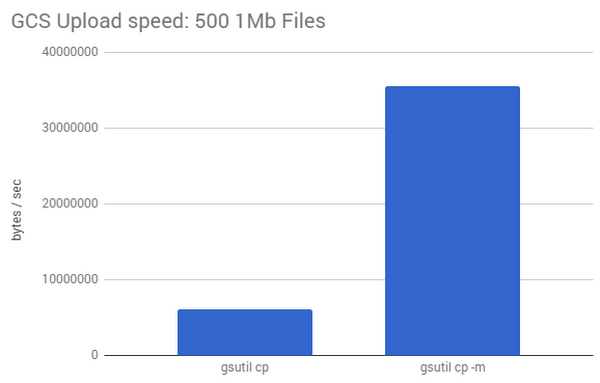
\includegraphics[width=12cm,keepaspectratio]{Pictures/cloud-storage-performance.png}
	\caption{GCS Uploadgeschwindigkeit in Bytes pro Sekunde, \citeurl{gcp-blog}}
\end{figure}

Hier sieht man, wie die Leistung sich dabei um das fünffache im Gegensatz zu den indivduellen Uploads erhöht. Das Auto-balancing von GC dient der Verteilung der Upload-Connections auf "Backend Shards". Das funktioniert durch  Name und Pfad der Datei und kann die Uploadgeschwindigkeit verringern, wenn sich die Dateien in unterschiedlichen Ordnern befinden oder verschiedene Namensgebungen haben. Falls sich die Dateien ähneln, kann dies die Uploadgeschwindigkeit erhöhen, da die Connections in den gleichen Shard übergehen.\\

Eine weitere Methode zur Performancesteigerung, sind Requests in Größen ab 1MB. Bei kleineren Requests sollten die Requests parallelisiert werden, damit die fixen Latenzkosten überlappt werden.\\
Es ist zu beachten, dass die Performance auch von anderen Faktoren abhängt, wie der Anwendungsarchitektur und der Netzwerkverbindung. Es können spezifische Konfigurationsoptionen genutzt werden, um die Leistung weiter zu optimieren, wie Caching, asynchrone Operationen oder die Nutzung von optimierten Bibliotheken oder Frameworks. 

\newpage

\subsubsection{API Anbindung}

\textbf{Amazon S3}\\

Die API-Anbindung von Amazon S3 ist umfangreich und bietet Entwicklern eine Vielzahl von Möglichkeiten zur Interaktion mit dem Speicherdienst. Amazon S3 bietet eine RESTful API (Application Programming Interface) sowie verschiedene SDKs (Software Development Kits) und Tools, welche die Integration und Nutzung erleichtern.\\

Mit der RESTful API, die auf dem HTTP-Protokoll basiert, können Entwickler HTTP-Anfragen wie GET, PUT, POST und DELETE verschicken, um auf Buckets und Objekte zuzugreifen, zu erstellen, zu lesen, zu aktualisieren und zu löschen. Amazon empfiehlt die Verwendung des AWS SDK, da bei Verwendung der REST API zusätzlicher Code zur Berechnung der gültigen Signatur für die Authentifizierung geschrieben werden muss. \glqq It requires you to write the necessary code to calculate a valid signature to authenticate your requests.\grqq, \cite{aws-api}.\\

Die Authentifizierung von Requests mit dem AWS SDK erfolgt durch die Bereitstellung von Access Keys, wodurch das Schreiben von Code dafür entfällt. Das SDK ist in verschiedenen Programmiersprachen verfügbar, darunter Java, JavaScript, Python, .NET, Ruby, PHP, iOS und Android. Die folgende Tabelle enthält eine Auflistung aller unterstützten Programmiersprachen:

\begin{table}[!h]
\centering
\begin{tabular}{ |p{5.5cm}|p{7cm}| }
\hline
\rowcolor{gray!30}
\textbf{SDK documentation} & \textbf{Code examples}\\
\hline
\textbf{AWS SDK for C++} & AWS SDK for C++ code examples\\
\textbf{AWS SDK for Go} & AWS SDK for Go code examples\\
\textbf{AWS SDK for Java}   & AWS SDK for Java code examples\\
\textbf{AWS SDK for Javascript}  & AWS SDK for Javascript code examples\\
\textbf{AWS SDK for Kotlin} & AWS SDK for Kotlin code examples\\
\textbf{AWS SDK for .NET} & AWS SDK for .NET code examples\\
\textbf{AWS SDK for PHP} & AWS SDK for PHP code examples\\
\textbf{AWS SDK for Python(Boto3)} & AWS SDK for Python(Boto3) code examples\\
\textbf{AWS SDK for Ruby} & AWS SDK for Ruby code examples\\
\textbf{AWS SDK for Rust} & AWS SDK for Rust code examples\\
\textbf{AWS SDK for Swift} & AWS SDK for Swift code examples\\
\hline
\end{tabular}
\caption{Unterstützte Programmiersprachen von AWS SDK, \citeurl{aws-sdk}}
\end{table}

Das SDK bietet eine Schnittstelle, um die Entwicklung von Anwendungen zu erleichtern und die Interaktion mit Amazon S3 zu vereinfachen. Darüber hinaus gibt es auch Drittanbieter-Tools und Open-Source Bibliotheken, welche die Integration mit Amazon S3 unterstützen. Spring Boot stellt eine Bibliothek für die alte und neue Version von AWS SDK zur Verfügung. IntelliJ Idea bietet den Plugin \verb|AWS Toolkit| an, mit dem Amazon Credentials zur Verfügung gestellt werden können. Dieses Plugin gibt es auch für Eclipse und Visual Studio Code.\\

Außerhalb des AWS SDK stellt Amazon S3 auch das AWS CLI (Command Line Interface) bereit, um API Aufrufe durchzuführen. Amazon S3 ermöglicht die Durchführung von Batch-Operationen, um mehrere Objekte in einem einzigen API-Aufruf zu verarbeiten. Dies erleichtert die effiziente Verarbeitung großer Datenmengen und reduziert die Anzahl der API-Anfragen.\\

Die API-Anbindung von Amazon S3 erfordert eine geeignete Authentifizierung und Autorisierung. Dies erfolgt in der Regel mithilfe von Zugriffsschlüsseln, die über AWS Identity and Access Management (IAM) verwaltet werden.

\newpage

\textbf{Google Cloud Storage}\\

Auch GC Storage bietet umfangreiche API-Integrationen, um die Einbindung in eigene Anwendungen zu ermöglichen. Eine davon sind die Client Libraries für verschiedene Programmiersprachen wie Java, Python, Node.js, Go, Ruby und .NET. Diese Bibliotheken erleichtern die Integration von GC Storage in Anwendungen und bieten eine benutzerfreundliche Schnittstelle für die Interaktion mit den Speicherressourcen. Auch bei Cloud Storage wird eine RESTful API ähnlich wie in Amazon S3 angeboten. Diese ermöglicht Entwickler, über HTTP-Anfragen auf die Speicherressourcen zuzugreifen. Sie unterstützt CRUD Operationen für Buckets und Objekte sowie erweiterte Funktionen wie das Setzen von Metadaten, das Verwalten von Zugriffssteuerungen und das Durchführen von Batch-Anfragen.\\

Google Cloud Storage bietet sowohl JSON- als auch XML-APIs für die Interaktion mit dem Speicherdienst. Neben der direkten API-Anbindung stellt Google auch das GC SDK zur Verfügung, das verschiedene Befehlszeilentools enthält, mit denen auf Speicherressourcen zugegriffen und verwaltet werden kann. Neben den Client-Bibliotheken werden auch Tools wie \verb|gsutil| (ein Befehlszeilen-Dienstprogramm) bereitgestellt. Dies ermöglicht, Cloud Storage von der Befehlszeile aus zu verwalten. Cloud Storage FUSE ermöglicht, Cloud Storage als Dateisystem zu mounten und direkt darauf zuzugreifen.\\

Die API-Anbindung von GC Storage erfordert ebenfalls eine Authentifizierung und Autorisierung. Dies wird mithilfe von GC IAM (Identity and Access Management) verwaltet, das Zugriffsrichtlinien und Rollenverwaltung bietet, ähnlich wie bei AWS.\\

Mit Terraform können Konfigurationen von GC Storage Buckets und Amazon S3-Buckets und die dazugehörigen Einstellungen in einer Terraform-Konfigurationsdatei spezifiziert werden. Diese Konfigurationsdatei enthält Informationen wie den Bucket-Namen, Zugriffsrechte, Verschlüsselungs-optionen und andere relevante Parameter. Terraform ist ein sogenanntes Infrastructure-as-Code-Tool, mit dem Infrastrukturressourcen in verschiedenen Cloud-Umgebungen, einschließlich GC und AWS, automatisiert erstellt und verwaltet werden können. Terraform sendet erforderliche API-Anfragen an GC oder AWS um den Bucket entsprechend der Konfiguration zu erstellen oder zu aktualisieren. Durch die Verwendung von Terraform für beide Cloud Provider kann die Infrastruktur als Code behandelt werden, wodurch die Konfiguration wiederholbar, versionierbar und leicht reproduzierbar wird. Auch können die Vorteile der Funktionen von Terraform genutzt werden, wie z.B. die Verwaltung von Abhängigkeiten zwischen Ressourcen, die Verwendung von Variablen und Modulen sowie die Integration in CI/CD-Pipelines.

\newpage

\subsection{Bereitstellung der Dateien}

In diesem Abschnitt werden Methoden für die Bereitstellung der Dateien durch signierte URLs von Amazon S3 und Cloud Storage präsentiert. Unternehmen und Organisationen stehen vor der Herausforderung, Dateien sicher und effizient für ihre Benutzer bereitzustellen. Eine häufig dafür verwendete Methode, ist die Verwendung signierter URLs. Diese ermöglichen es, auf einfache Weise temporäre Zugriffsrechte für Dateien zu gewähren, ohne komplexe Zugriffskontrollmechanismen implementieren zu müssen. Sowohl AWS S3 als auch GC Storage bieten die Möglichkeit, signierte URLs für die Dateibereitstellung zu generieren. Beide bieten ähnliche Funktionen an, signierte URLs durch die SDKs zu generieren. \\

\textbf{Amazon S3}\\

In Amazon S3 sind alle Objekte und Buckets standardmäßig privat. Durch die Verwendung von presigned URLs können Objekte bereitgestellt werden, ohne die Voraussetzung, ein AWS Konto zu besitzen. \glqq All objects and buckets are private by default. However, you can use a presigned URL to share objects with others.\grqq, \cite{aws-signed-urls}. 

\begin{quote}
	Presigned URLs werden für die Generierung von Links verwendet, um auf S3 Buckets und Objekte zugreifen zu können. Bei der Erstellung solcher URLs können andere Nutzer von außerhalb AWS ohne Credentials auf die gewünschten Daten zugreifen. Jeder, der diesen Link hat, kann darauf zugreifen und Aktionen ausführen. Der Link verliert je nach Konfiguration nach einer bestimmten Zeit die Gültigkeit. Amazon S3 überprüft das Verfallsdatum des Links während des HTTP Requests, vgl. \cite{aws-signed-urls}. 
\end{quote}

Durch die Nutzung der URL können Nutzer Objekte lesen oder hochladen. In Fall von leoticket liegt das Lesen des Objekts im Fokus. Die URL beinhaltet spezielle Parameter, welche von einer Anwendung gesetzt werden. Es gibt drei Parameter, um den Zugriff für den Nutzer einzuschränken. Diese sind einmal Einschränkung des Buckets. Das bedeutet, das ein Nutzer nicht auf jeden Bucket zugreifen kann, sondern nur auf den Bucket, indem sich das Objekt befindet. Der zweite Parameter ist der Name des Objekts und zuletzt die Zeitspanne in der die URL gültig ist. Sobald die Zeit abgelaufen ist, kann der Nutzer nicht mehr auf den Link zugreifen.\\

Durch die Methode der presigned URLs können diese Links über die Email an die Clients versendet werden. Somit kann die Bereitstellung der erfassten Daten des Produkts leoticket über die presigned URLs stattfinden und Email-Anhänge vermieden werden.

\newpage

\textbf{Google Cloud Storage}\\

In GC Storage funktioniert die signed URL gemäß einem ähnlichen Prinzip wie in Amazon S3. Durch zeiteingeschränkte Links können Nutzer, welche den Link besitzen, ohne GC Credentials auf Objekte und Buckets zugreifen. Dabei bietet Cloud Storage mehrere Methoden zur Generierung einer Signed URL an. Die V4 signing with service account authentication, Signing with HMAC authentication und die V2 signing with service account authentication, vgl.\footcite{gc-signedUrl}. Letztere Methode wird ausgeschlossen, da sie von GC selbst nicht empfohlen wird. Ein Beispiel, wie eine signierte URL aussehen kann:

\begin{lstlisting}
	https://storage.googleapis.com/[BUCKET_NAME]/[OBJECT_NAME]?GoogleAccessId=[SERVICE_ACCOUNT_EMAIL]&Expires=[EXPIRATION_TIMESTAMP]&Signature=[URL_SIGNATURE]
\end{lstlisting}

Hierbei sind die Platzhalter wie folgt zu ersetzen:

\begin{itemize}
	\item BUCKET\_NAME - Der Name des GCS-Buckets, in dem sich das Objekt befindet.
	\item OBJECT\_NAME - Der Name des Objekts, für das die signierte URL generiert werden soll.
	\item SERVICE\_ACCOUNT\_EMAIL - Die E-Mail-Adresse des Service Accounts, der die Zugriffsberechtigung hat.
	\item EXPIRATION\_TIMESTAMP - Das Ablaufdatum der signierten URL in Form eines Unix-Timestamps.
	\item URL\_SIGNATURE - Die Signatur der URL, die den Zugriff autorisiert.
\end{itemize}

Im Vergleich zu AWS unterscheiden sich die Parameter bei der Zugriffsberechtigung. In AWS wird der \verb|ACCESS_KEY_ID| statt der Service Account Email verwendet. Die Access Key ID ist dabei der Zugriffschlüssel des AWS-Kontos, das die Zugriffsberechtigung hat.

\newpage

\section{Auswahl des Speichersystems}

In diesem Kapitel werden anhand der Anforderungen von leoticket die Kostenanalyse durchgeführt und Konfigurationseinstellungen empfohlen.

\subsection{Kostenanalyse}

Bei der Kostenanalyse werden die Gebühren aus dem Kostenabschnitt (2.2.1.3) übernommen und eine Kostenabschätzung für Amazon S3 und Cloud Storage durchgeführt. Es werden die Kosten für die Speicherung, das Abrufen und die Datenübertragung verglichen und dargestellt. Die Berechnungsdaten sind exemplarisch ausgewählt und dienen der groben Kosteneinschätzung. Dabei wurden die aktuellsten Gebühren aus der offiziellen Dokumentation von AWS und GC übernommen.\\

Für eine grobe Kosteneinschätzung wird von durchschnittlich 800 000 Bestellungen pro Jahr ausgegangen. Dies entspricht etwa 67.000 Bestellungen pro Monat , wobei jede Bestellung 4 Objekte enthält. Die durchschnittliche Größe eines Objektes beträgt dabei 100 KB. Für jede  Bestellung wird von durchschnittlich drei Ticketkäufen ausgegangen, bei denen eine zusätzliche Rechnung hinzugefügt wird. Dadurch werden monatlich etwa 268.000 POST-Anfragen an Buckets verschickt. Außerdem wird erwartet, dass Objekte zweimal im Monat von leoticket Kunden abgerufen werden. Insgesamt wird es 536.000 GET-Anfragen geben. Es ist zu beachten, dass jedes Objekt einzeln hochgeladen wird.\\

Die Speichergröße wird durch die Multiplikation der Anzahl von 67.000 Bestellungen pro Monat mit der Größe von 400 KB pro Bestellung ermittelt. Dieses Ergebnis wird durch 1024 geteilt und das resultierende Ergebnis erneut durch 1024 geteilt, um die Größe in GB zu erhalten. Dies ergibt eine monatliche Speichergröße von 25 GB. Unter Berücksichtigung einer Aufbewahrungsdauer von 10 Jahren ergibt sich eine geschätzte Datenmenge von etwa 3 TB, wenn die Daten nach 10 Jahren gelöscht werden. Für die Preisberechnung werden diese Daten in die \href{https://calculator.aws/#/addService?nc2=h_ql_pr_calc}{AWS Preisrechner} und \href{https://cloud.google.com/products/calculator}{GC Preisrechner} eingesetzt.\\

\newpage

\textbf{Amazon S3}\\

Im Folgenden stellt die Tabelle die monatlichen Kosten der verschiedenen Speicherklassen dar. Die Vorabkosten, die unten berechnet werden, müssen an AWS gezahlt werden:

\begin{table}[!h]
\begin{tabular}{ |s|p{2cm}|p{2.5cm}|p{2cm}|p{2cm}| }
\hline
\rowcolor{blue!35}
 & \textbf{Standard} & \textbf{Intelligent Tiering} & \textbf{Standard-IA} & \textbf{One Zone-IA}\\
\hline
\textbf{Speicherkosten} & 70,27 EUR & 70,27 EUR & 38,72 EUR & 30,98  EUR \\
\textbf{Vorabzahlung} & 162,42 EUR & 162,42 EUR & 300,76 EUR & 300,76 EUR \\
\textbf{PUT Requests}   & 1,35 EUR & 1,35 EUR  & 2,50 EUR & 2,50 EUR\\
\textbf{GET Requests}  & 0,22 EUR & 0,22 EUR  & 0,50 EUR & 0,50 EUR\\
\textbf{Datenabrufe} & -- & -- & 0,47 EUR & 0,47 EUR\\
\hline
\textbf{Data Transfer} & \multicolumn{3}{c}{4,20 EUR} &\\
\hline
\textbf{Monitoring und Automation objects} & -- & 75,19 EUR & -- & --\\
\hline
\end{tabular}
\caption{Übersicht der einzelnen Kosten der Datenspeicherung in Amazon S3}
\end{table}

Zunächst werden die Einheitsumwandlungen durchgeführt. Hierbei wird die angegebene Datenmenge von 3 TB pro Monat mit 1024 GB multipliziert, um die genaue Menge in GB zu berechnen. Das ergibt einen Wert von 3072 GB. Daraufhin wird die Objektgröße von 100 KB in GB umgerechnet, was einem Wert von 0,000095367432 GB entspricht. Anschließend werden die Preise anhand dieser berechneten Werte ermittelt:

\begin{align}
	\frac{3072 \text{ GB per Month}}{0,000095367432 \text{ GB average item size}} = 32.212.255 \text{ number of objects}\\
	3072 \text{ GB} \times 0,013 \text{ EUR} = \text{38,72 EUR Standard-IA costs}\\
	268.000 \text{ PUT requests} \times 0,0093 \text{ EUR per request} = 2,50 \text{ EUR (PUT requests cost)}\\
	536.000 \text{ GET requests} \times 0,00093 \text{ EUR per request} = 0,50 \text{ EUR (GET requests cost)}\\
	50 \text{ GB} \times 0,00093 \text{ EUR} = 0,47 \text{ EUR (data retrievals cost)}\\
	38,72 \text{ EUR} + 2,50 \text{ EUR} + 0,50 \text{ EUR} + 0,47 \text{ EUR} = \underline{\textbf{42,19  EUR (Total Standard-IA)}}\\
	32.212.255 \text{ number of objects} \times 0,0000093 \text{ EUR} \\ = \text{300,76 EUR (Cost for PUT, COPY, POST requests for initial data)}
\end{align}

Die oben genannten Formeln ähneln denen für die Speicherklassen Standard und One Zone-IA, wobei die entsprechenden Gebühren aus dem Kostenabschnitt übernommen wurden. Bei der Intelligent Tiering gibt es jedoch einen Unterschied: Es fallen zusätzliche Kosten für Überwachung und Automatisierung an, und der Speicher wird in drei Klassen prozentual aufgeteilt. In der letzten Zeile der Tabelle werden die Gesamtkosten zusammen mit den Kosten für den Datentransfer, eventuelle Vorauszahlungen (zusätzlich in 3.8) und die reinen monatlichen Speicherkosten für die jeweiligen Speicherklassen addiert.

\newpage
\textbf{GC Storage}\\

Die nachstehende Tabelle stellt eine Zusammenfassung der monatlichen Kosten für drei Speicherklassen von GC Storage dar:

\begin{table}[!h]
\centering
\begin{tabular}{ |s|p{2cm}|p{2cm}|p{2cm}| }
\hline
\rowcolor{green!25}
 & \textbf{Standard} & \textbf{Nearline} & \textbf{Coldline}\\
\hline
\textbf{Speicherkosten} & 63,75 EUR & 36,03 EUR & 16,63 EUR\\
\textbf{Datenabrufe} & -- & 0,45 EUR & 0,90 EUR\\
\textbf{Klasse A Operationen}   & 1,21 EUR & 2,42 EUR  & 4,84 EUR\\
\textbf{Klasse B Operationen}  & 0,19 EUR & 0,48 EUR   & 4,84 EUR\\
\hline
\textbf{Internet Egress} & \multicolumn{2}{c}{3,83 EUR pro 0 bis 1TB} &\\
\hline
\end{tabular}
\caption{Übersicht der einzelnen Kosten der Datenspeicherung in GC Storage}
\end{table}

Die Speicherklasse mit den höchsten Kosten von 63,75 Euro ist die Standardklasse. Die Coldlineklasse ist die kostengünstigste Option mit Kosten von 16,63 Euro. Die Nearlineklasse ist teurer als die Coldlineklasse und kostet 36,03 Euro. In der Standardklasse fallen keine Gebühren für den Datenabruf an, während für Nearline 0,45 Euro und für Coldline 0,90 Euro berechnet werden. In Klasse A ist die Nearlineklasse mit 2,42 Euro doppelt so teuer wie die Standardklasse, während die Coldlineklasse mit 4,84 Euro doppelt so teuer wie die Nearlineklasse ist. In Klasse B ist die Standardklasse mit 0,19 Euro am günstigsten, während die Nearlineklasse etwa doppelt so teuer ist. Die Coldlineklasse ist hier etwa zehnmal teurer als die Nearlineklasse. Für den Internet-Ausgangsverkehr fallen Gebühren von 3,83 Euro pro 0 bis 1 TB monatlich an. Die Tabelle zeigt, dass die Standardklasse doppelt so teuer ist wie die Nearlineklasse und etwa dreimal so teuer wie die Coldlineklasse. Die Preise ergeben sich durch die unterschiedlichen Anwendungsfälle der Speicherklassen, die in der Entscheidungsfindung genauer erklärt werden.                            

\newpage

\subsection{Entscheidungsfindung} 

Um der Anforderung der sicheren Speicherung des Produkts leoticket zu entsprechen, bieten beide Cloud Provider Funktionen an, die im vorherigen Kapitel unter Eigenschaften untersucht worden sind. Beide Cloud Provider bieten ähnliche Funktionen für die Erstellung von Benutzern, Gruppen und Rollen, um den Zugriff auf die Dienste einzuschränken. Die IAM Funktionen beider Cloud Provider ermöglichen die Beschränkung des Zugriffs auf S3 und Cloud Storage. Bei der IAM-Funktion in AWS S3 werden Vorgehensweisen empfohlen, um die Sicherheit und den Zugriff auf S3-Ressourcen zu verbessern. Beispielsweise das Prinzip des geringsten Privilegs. Benutzern und Anwendungen sollten nur die Berechtigungen, die sie zum Durchführen ihrer Aufgaben benötigen, gewährt werden. Überflüssige Berechtigungen sollten vermieden werden. Das beinhaltet beispielsweise Schreib- und Leseberechtigungen für Objekte. Es können auch andere Berechtigungen, wie das Hinzufügen von Richtlinien, vergeben werden. Diese Empfehlung gilt auch für die IAM-Funktion in GC. Für die Authentifizierung von Anwendungen stehen Service Accounts zur Verfügung, die spezifische Berechtigungen haben, welche für die Anwendung relevant sind. Für jeden Dienst oder jede Anwendung kann ein eigener Service Account erstellt werden.\\

Auch bei der Datenverschlüsselung bieten beide Cloud Provider ähnliche Möglichkeiten, mit Encryption Keys umzugehen. Da leoticket eine sichere Speicherung erfodert, kommt die SSE-KMS customer-managed Variante in Frage. Durch die selbstständige Generierung des Schlüssels und Verwaltung hat der Nutzer im Gegensatz zu S3-managed oder Google-managed Keys mehr Kontrolle. Die generierten Schlüssel werden jedoch vom Cloud-Anbieter im KMS gespeichert. Wenn die Option SSE-KMS gewählt wird, kann die Funktion Bucket Keys in S3 aktiviert werden. Dadurch wird ein Master Key verwendet, der die Schlüssel der einzelnen Objekte verschlüsselt. Dies führt zu einer Reduzierung der Request-Kosten um bis zu 99 Prozent, da der Request-Verkehr von S3 zu AWS KMS verringert wird.\\

Um eine größere Unabhängigkeit vom Cloud-Anbieter zu gewährleisten, kann die Option customer-managed in S3 in Betracht gezogen werden.In diesem Fall trägt der Nutzer die volle Verantwortung für die Schlüssel. Das bedeutet, dass die Schlüssel extern vom Nutzer generiert, verwaltet und gespeichert werden. Es besteht jedoch das Risiko, dass der Schlüssel verloren geht und der Zugriff auf die Objekte in S3 oder Cloud Storage nicht mehr möglich ist. Darüber hinaus erfordert die eigenständige Verwaltung des Schlüssels einen höheren Aufwand im Vergleich zur Verwendung des KMS. Bei der Erstellung von signierten URLs müssen folgende Encryption Header der Request angehängt werden: 

\begin{table}[!h]
\centering
\begin{tabular}{ |p{5cm}|p{8cm}| }
\hline
Name & Description \\
\hline
\cline{1-2}
x-amz-server-side-encryption-customer-algorithm & Use this header to specify the encryption algorithm. The header value must be AES256.\\
\cline{1-2}
x-amz-server-side-encryption-customer-key & Use this header to provide the 256-bit, base64-encoded encryption key for Amazon S3 to use to encrypt or decrypt your data. \\
\cline{1-2}
x-amz-server-side-encryption-customer-key-MD5 & Use this header to provide the base64-encoded 128-bit MD5 digest of the encryption key according to RFC 1321. Amazon S3 uses this header for a message integrity check to ensure that the encryption key was transmitted without error.\\
\cline{1-2}
\end{tabular}
\caption{Benötigte Encryption Header für signierte URLs mit SSE-C, \cite{aws-sse-c} }
\end{table}

\newpage

Die Implementierung von signierten URLs in Verbindung mit customer-supplied Encryption Keys ist in der offiziellen Dokumentation von GCP nicht enthalten.\\

Beide Cloud-Anbieter bieten die Möglichkeit, ACLs auf Objekte und Buckets anzuwenden. Es wird jedoch empfohlen, ACLs auf Objektebene standardmäßig deaktiviert zu lassen und nur in Fällen zu verwenden, in denen der Uploader eines Objekts die vollständige Kontrolle über diese und auf andere Objekte eingeschränkten Zugriff in einem Bucket hat.\\

Um die Sicherheit und Verfügbarkeit von Daten zu gewährleisten, wird empfohlen, die Objektversionierung zu aktivieren, um mehrere Versionen von Objekten zur Verfügung zu stellen. Dadurch können Objekte bei versehentlichem Löschen oder Überschreiben wiederhergestellt werden. Diese Funktion wird von beiden Cloud-Providern angeboten und kann beim Erstellen eines Buckets aktiviert werden.\\

AWS und GC stellen eine Auswahl verschiedener Speicherklassen zur Verfügung. Beide Anbieter garantieren eine Verfügbarkeit von mindestens 99,5\%. Die Speicherklassen Standard-IA und One Zone-IA bieten kostengünstigere Optionen für die Datenspeicherung. Die Standard-IA eignet sich für Daten, auf die seltener zugegriffen wird, die aber bei Bedarf schnell verfügbar sein müssen. Im Vergleich zur Standardklasse sind die Speicherkosten niedriger, jedoch fallen zusätzliche Gebühren für den Datenabruf an. Wenn Daten zwischen zwei Speicherklassen verschoben werden, entstehen Kosten für den Wechsel der Speicherklassen, die von der verschobenen Datenmenge abhängen.\\

Die Speicherklasse One Zone-IA eignet sich für Daten, auf die selten zugegriffen wird, weist jedoch eine Einschränkung auf. Im Gegensatz zu den anderen Speicherklassen wird One Zone-IA nur in einer einzigen Verfügbarkeitszone (AZ) in einer bestimmten Region gespeichert. Das bedeutet, dass die Daten nur in dieser einen AZ verfügbar sind und das Risiko besteht, dass die Daten nicht zugänglich sind, wenn diese spezifische AZ nicht verfügbar ist.

\newpage

Für leoticket werden die Speicherklassen Standard-IA von S3 und Nearline von Cloud Storage empfohlen. Da in leoticket eine schnelle Dateiabfrage innerhalb von Millisekunden erforderlich ist, kommen die Speicherklassen von S3 Glacier nicht in Betracht, da das Abrufen von Dateien in diesen Speicherklassen Tage oder Stunden dauern kann. Die Archive Storage Klasse von GCP kommt ebenfalls nicht in Betracht, da der Prozess des Datenabrufs, um die Dateien wieder zugänglich zu machen, mehrere Sekunden dauern kann. In diesem Prozess werden die Daten vom Archive Storage zum Online Storage verschoben.\\ 

Die Daten in leoticket müssen jederzeit abrufbereit sein, jedoch wird davon ausgegangen, dass Objekte im Durchschnitt nur zweimal von leoticket Kunden abgerufen werden. Aufgrund der geringen Anzahl von Abrufen pro einzelner Objekte und der erforderlichen Speicherung von Daten über einen Zeitraum von 10 Jahren sind die Speicherklassen Standard-IA und Nearline geeignete Optionen. Diese Speicherklassen sind für Daten ausgelegt, auf die seltener zugegriffen wird, aber bei Bedarf dennoch schnell verfügbar sein müssen. Sie bieten eine kostengünstigere Möglichkeit zur Speicherung der Daten, denn die Speicherung ist günstiger als bei den Standard Klassen.\\ 

Die Speicherklasse One Zone-IA von S3, welche die Daten nur in einer einzigen AZ speichert, wird aufgrund des Risikos einer eingeschränkten Verfügbarkeit bei Ausfall dieser spezifischen AZ nicht empfohlen. Dadurch kann sich die Zeit für den Abruf von Daten verlängern. Die Abrufkosten sind ebenfalls höher als bei anderen Speicherklassen, da diese Klasse nicht für Daten ausgelegt ist, auf die mindestens zweimal zugegriffen werden muss.\\ 

Die Coldline-Speicherklasse von GC kann in Betracht gezogen werden, wenn Daten für eine längere Zeit nicht abgerufen wurden und auch in naher Zukunft nicht erwartet wird, dass sie wieder abgerufen werden. Diese Speicherklasse ist für Daten geeignet, auf die selten zugegriffen wird und bei denen eine längere Zugriffszeit akzeptabel ist. Sie eignet sich gut für die Archivierung von Daten. Hier könnte auf die Auto-Class Funktion von GC oder auf die Intelligent-Tiering von AWS zugegriffen werden, um Dateien automatisch in die passenden Speicherklassen zu verschieben. Jedoch fallen auch hier Gebühren bei der Nutzung dieser Funktionen an.\\


Im Hinblick auf die API-Integration gibt es einige Unterschiede zwischen den beiden Providern. Für leoticket ist es relevant, dass die API nahtlos in die leoticket-Anwendung integriert werden kann, ohne großen Aufwand betreiben zu müssen. Beide Anbieter bieten geeignete SDKs, CLIs und REST APIs an, die problemlos in die eigene Anwendung eingebunden werden können. Es gibt auch Frameworks wie Spring Boot, die Bibliotheken für sowohl die AWS SDK-Version 1 und 2 als auch für GC bereitstellen.\\ 

Ein Vorteil von AWS besteht darin, dass On-Premise-Anwendungen wie MinIO die AWS API verwenden und somit eine Kompatibilität mit S3 gewährleisten. Anwendungen oder Skripte können so konfiguriert werden, dass sie die S3 API verwenden, um mit MinIO zu interagieren. Die API-Endpunkte und Authentifizierungsmechanismen sind mit der S3 API kompatibel, was bedeutet, dass S3 Anwendungen auf MinIO umgestellt werden können.

\newpage 

GC kann ebenfalls mit MinIO integriert werden. Dabei dient MinIO als Gateway. Nach den nötigen Konfigurationen kann auf GC Storage über den MinIO Server Endpoint zugegriffen werden. Dabei wird das Standard AWS S3 SDK für die Integration mit Cloud Storage verwendet. Jedoch erfordert es eine Einarbeitung in das AWS SDK als GC Storage Nutzer.\\ 

Für die Authentifizierung mit der API bei GC wird empfohlen, die Verwendung von Service Accounts aus dem Google SDK zu nutzen. Es gibt jedoch auch andere Methoden zur Authentifizierung, und über Application Default Credentials (ADC) in GC kann die bevorzugte Methode festgelegt werden. AWS bietet das \verb|AWS Toolkit| zur Authentifizierung an, das von IntelliJ Idea, Eclipse und anderen IDEs unterstützt wird. Die Verwendung des Toolkits wird zur Authentifizierung empfohlen. Insgesamt bieten sowohl AWS als auch GC gute Möglichkeiten zur API-Integration, wobei spezifische Faktoren wie Vorwissen, vorhandene Technologien und Anforderungen berücksichtigt werden sollten.\\

Um eine optimale Performance für leoticket zu gewährleisten, empfiehlt es sich, Performance-Analysen durchzuführen. Sowohl AWS als auch GC bieten Tools zur Unterstützung an. Bei GC kann die Performance-Diagnose mithilfe des \verb|gsutil| CLI durchgeführt werden. Dies ist auch erforderlich, wenn der Support von GC kontaktiert wird, um bei der Fehlerbehebung zu helfen. AWS hingegen bietet im S3-Bucket Metriken an, die zur Performance-Analyse genutzt werden können. Es werden verschiedene Widgets für Request-Metriken bereitgestellt, die analysiert werden können. AWS hat jedoch keine speziellen Performance-Analyse Tools wie das \verb|gsutil perfdiag| von GC. Im Kapitel \glqq Prototypische Umsetzung\grqq\ werden Performance-Messungen durchgeführt und anschließend analysiert, um einen besseren Vergleich der beiden Cloud-Anbieter in Bezug auf die Performance zu ermöglichen. Es ist ratsam, diese Analysen regelmäßig durchzuführen, um mögliche Leistungsprobleme frühzeitig zu erkennen und zu optimieren.\\ 

Die Entscheidung zwischen den Cloud Providern hängt sowohl von den Anforderungen von leoticket als auch von den Präferenzen der Entwickler ab. Wenn Entwickler bereits Erfahrung und Kenntnisse mit einem bestimmten Cloud Provider haben, ist es ratsam, sich für diesen Provider zu entscheiden. Dies bietet den Vorteil, dass man sich nicht in eine neue Technologie einarbeiten muss und Zeit bei der Implementierung und Integration der API sparen kann. Es ist durchaus legitim zu sagen, dass beide Anbieter eine Vielzahl von Funktionen und ähnlichen Produkten anbieten, die an die Anforderungen von leoticket angepasst werden können. Diese Arbeit soll lediglich als Leitfaden dienen, um bei der Entscheidung zu unterstützen und letztendlich eine fundierte Wahl zu treffen.